\documentclass[12pt, a4paper]{article}
\usepackage[utf8]{inputenc}
\usepackage{graphicx}
\usepackage{geometry}

\setlength\parindent{0pt} % No indent
\setlength{\parskip}{1em} % Space between paragraphs

\title{
    \begin{flushleft}
        {\huge [Game name]: \textbf{User manual}} \\
        \vspace{0.5cm}
        \large\emph{Software Engineering Project (DAT255/DIT543)} \\
        \large\emph{Chalmers tekniska Högskola} \\
        \vspace{0.5cm}
        Group: G257 \\
        \vspace{0.5cm}
        {\rule{\linewidth}{0.5mm}}
        \end{flushleft}
        \vspace{1cm}
}
\author{}
\date{}

\begin{document}

\maketitle

\section{Introduction}
\textit{game name} is for the travelling gamer who desires a challenge during his/her daily commute. We offer several exciting stages to conquer with a variation of difficulty. You take the role of an adventurer ready to explore the lands and reach the end goal of traveling the lands and all the danger within them. The game is in the style of a classic 2D side controller fashion where the player travels along the landscape. The stage is completed by reaching the goal at the end of the stage.

\newpage

\section{Guide}
This guide will show you the main features of this game.

\section{Start menu}
When the app start the first thing you will see is the main menu. Three buttons are displayed in the menu: \textit{Start}, \textit{Level Select} and \textit{High Score}. Be selecting \textit{Start} you will be taken to the first level. If you want to choose a specific level then press \textit{Level Select}. The start menu is shown in Figure~\ref{fig:startmenu}.

\begin{figure}[ht!]
    \centering
    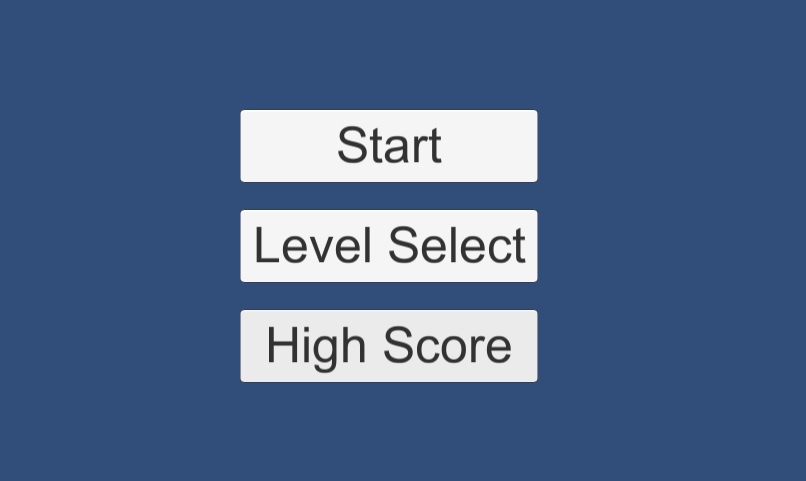
\includegraphics[width=8cm]{startmenu.jpg}
    \caption{The start menu.}
    \label{fig:startmenu}
\end{figure}

\subsection{Level Select}
When the \textit{Level Select}-button is selected from the start menu a level select menu will be shown. Every group member has created their own set of levels. By swiping left or right you can choose which group members levels you want to see. This menu is shown i Figure~\ref{fig:levelselect}.

\begin{figure}[ht!]
    \centering
    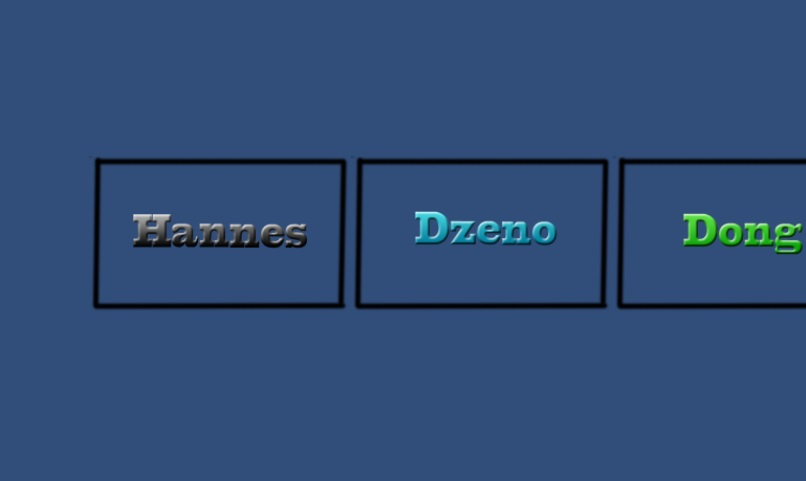
\includegraphics[width=8cm]{levelselect.jpg}
    \caption{The Level select menu.}
    \label{fig:levelselect}
\end{figure}

When a group members button is pressed the screen will rotate 90 degrees and the group members levels will be shown. You can scroll between the levels by swiping to left or right. In Figure~\ref{fig:levelselect2} you can see how the screen looks.

\begin{figure}[ht!]
    \centering
    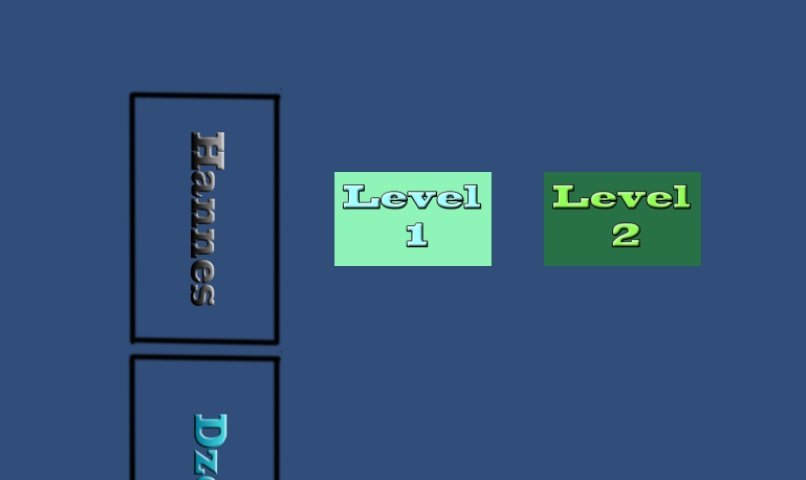
\includegraphics[width=8cm]{levelselect2.jpg}
    \caption{Hannes levels har shown.}
    \label{fig:levelselect2}
\end{figure}

\end{document}
